\documentclass[11pt,a4paper]{article}
\usepackage[utf8]{inputenc}
\usepackage{amsmath}
\usepackage{amsfonts}
\usepackage{amssymb}
\usepackage{graphicx}
\usepackage{array}
\usepackage{multirow}
\usepackage[margin=1cm]{geometry}
\usepackage[table]{xcolor}
\graphicspath{ {./images/} }
\author{Bianca}
\DeclareMathOperator*{\argmin}{argmin}
\DeclareMathOperator*{\diag}{diag}
\DeclareMathOperator*{\sign}{sign}
\begin{document}
\begin{flushleft}
\section{Begriffe}
\begin{table}[]
{\rowcolors{1}{black!10!}{black!5}
\begin{tabular}{l p{5cm} l p{7cm} l p{7cm}}
\textit{O} & is a set of objects  & Mushrooms \\
\textit{C} & is a set of classes  & essbar oder nicht \\
$X$ & Set/ Menge der Feature Vektoren & Vektoren mit den Eigenschaften der Pilze                 \\
\textbf{X}                                                             & Feature Vektor; Feature Space; Feature Domain                                      &                                                                                                                       \\
\textbf{x}                                                             & one feature vector                                                                 & ein Pilz                                                                                                              \\
x                                                                      & single feature                                                                     & ein eigenschaft von einem Pilz (z.B. braun)                                                                          \\
\textbf{w}                                                             & Weight-Vektor                                                                      &                                                                                                                       \\
$D={(x_1, c(x_1)),…, ((x_n, c(x_n))}$                         & classification knowledge alias the example set                                     & schon bestimmte Pilze                                                                                                 \\
\textit{D = \{(x1, y1), … , ((xn, yn)\}}                               & same but for regression                                                            & Mietpreise von Wohnungen                                                                                             \\
$\alpha(o) = x$                                                               & model formation function                                                           & Funktion zur Bestimmung der Pilz-Eigenschaften                                                                       \\
y(x) (Ziel y(x) = c(x))                                                & model function/ classifier                                                         & Bestimmung ob essbar anhand der Eigenschaften                                                                          \\
\textit{$\gamma(o)$ mit $O \rightarrow C$}                                                & ideal target function / ideal classifier für O                                     & Pilzexperte der Pilze bestimmt                                                                                         \\
c(x) mit c: $X \rightarrow C$                                                      & ideal target function/ ideal classifier for X ; indirekt gegeben durch D           & Theoretische Ideale Bestimmung aller Pilze                                                                            \\
$h(x), h: X \rightarrow \{0,1\}$                                                   & hypothesis/ model function  to approximate c(x)                                    & wenn es sonnig ist mache ich Sport (Regeln/ Hypothesen  zur classification)                                            \\
$y_i$                                                                     & ground truth for $xi \in X $                                                            & der Mietpreis für eine Wohnung                                                                                       \\
\textit{H}                                                             & hypothesis space                                                                   & Menge alle möglichen Hypothesen/Regeln                                                                                 \\
$VH,D = \{h(x) | h(x) \in  H \wedge $ & \multirow{2}{7cm}{version space : Menge aller möglichen Regeln (h(x)) die sich aus D ableiten lassen} & \multirow{2}{7cm} {Wenn es sonnig ist gehe ich raus, Wenn es warm ist gehe ich raus, wenn es windig ist und scheint gehe ich raus, etc.}  \\
$( \forall(x, c(x)) \in D : h(x) = c(x)) \}$ & &  \\
\textit{\#}                                                            & true error                                                                         & die summe aller falsch klassifizieren x durch Gesamtzahl aller x                                                       \\
\textit{$X \in X / C \in C$}                                                 & random variables                                                                   & ein random Pilz bzw. eine random Klasse                                                                              \\
$p(x, c) = P(X=x, C=c)$                                                  & the probability of the joint event that $x \in X$ \& x belongs to class $c \in C   $ & die Wahrscheinlichkeit das ein Pilz zu einer bestimmten Klasse gehört                                                  \\
$\eta$                                                                      & {learning rate}                                                                & a small positiv constant                                                                                              \\
                                                                       & p- dimensional direction vector $w \rightarrow = (w1, . . . , wp) T$ &                                                                                                                       \\
                                                                       & p + 1)-dimensional hypothesis $w = (w0, w1, . . . , wp) T$                                                                                                                                             & 
\end{tabular}
}
\end{table}
\section{Definition Formel \& Algorithmen}

\subsection{Specification of learning tasks}
    \textbf{Realworld $\rightarrow$ Modelworld} \newline
    \begin{enumerate}
    \item \textbf{Reale Welt:}
    \end{enumerate}
    \begin{itemize}
        \item $O$ - Menge an Objekten
        \item $C$ - Menge an Klassen
        \item $\gamma: O \rightarrow C$ - idealer Classifier für $O$
    \end{itemize}
    \quad Aufgabe-Klassifizierung:
    \begin{itemize}
        \item bestimme von $o \in O$ die Klasse $\gamma(o) \in C$
    \end{itemize}
    
    \begin{enumerate}
        \setcounter{enumi}{1}
        \item \textbf{Model Welt}
    \end{enumerate}
     \begin{itemize}
         \item $X$ - Menge von feature Vektoren
         \item $C$ - Menge von Klassen
         \item $c: X \rightarrow C$ - idealer Classifier für $X$ \textit{(c ist unbekannt)}
         \item $ D =$ \{($\textbf{x}_1,c(\textbf{x}_1)),\ \dots\ ,(\textbf{x}_n, c( \textbf{x}_n)) $\} - Menge von Beispielen \textit{(bereits klassifiziert)}
     \end{itemize}
    Todo: Schätze $c(\mathbf{x})$, welche implizit durch $D$ gegeben sind, durch
    \newline \quad Model-Funktion $y(\mathbf{x})$ 
    \newline\newline
    Machine Learning: \newline
    \begin{enumerate}
        \item Formuliere Model-Function: $y: X \rightarrow C, \mathbf{x} \mapsto y(\mathbf{x})$
        \item Nutze Statistik, Theorie und Algorithmen aus ML um den fit zwischen $c(\mathbf{x})$ und $y(\mathbf{x})$ zu Maximieren
    \end{enumerate}
    \includegraphics[width=\textwidth]{modelworld}
    
    \subsection{LMS: Least Mean Squared}
    Ziel: Fitting $y(x)$; Anpassung der weights, sodass Klassifizierungsfehler möglichst gering sind. \\~\\
    Input: $D$ - Trainingsdaten ($\mathbf{x},c(\mathbf{x})$) mit \textbf{x}$\in \textbf{R}^p$ und Zielklasse c(\textbf{x}) 
    $\eta$ Learning rate, kleine positive Konstante
    \\~\\
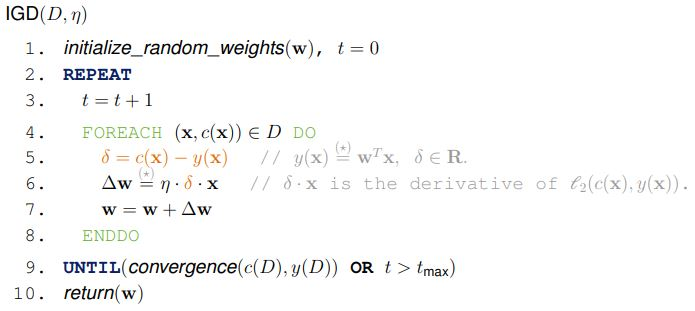
\includegraphics[width=\textwidth]{IGD}

\subsection{Lineare Regression}

Grundformel für lineare Gerade, mit: \newline
$y(x)$ - abhängige Variabel
$x$ - unabhängige Variable
$w_1$ - Anstieg der Geraden
$w_0$ - Schnittpunkt der y-Achse
\begin{equation}
    y(x)=w_o+w_1\cdot x
\end{equation}
Wobei das minimale $w_0$ und $w_1$ sich ergeben aus:
\begin{equation}
    w_1=\frac{\sum\limits^{n}_{i=1}(x_i-\overline{x}\cdot(y_i-\overline{y})}{\sum\limits_{i=1}^{n}(x_i-\overline{x}^2}
\end{equation}
\begin{equation}
    w_0=\overline{y}-w_1\cdot\overline{x}
\end{equation}

\paragraph{Goodness of Modelfit, Regressionserror}
Residual sum of Squares(RSS). \newline
Der Residue wird aus der Differenz zwischen (beobachteten) Realwelt-Wert $y_i$ und geschätzten/modelierten Wert $y(\mathbf{x}_i)$
\begin{equation}
    RSS(\mathbf{w}) = \sum^{n}_{i=1}(y_i-y(\mathbf{x}_i))^2
\end{equation}

\paragraph{Higher-Dimensional Feature Space} ML:ll-16


\subsection{Concept Learning}
Setting:\newline
$X$ - Menge an Feature Vektoren\newline
$C$ - Ist eine Menge mit zwei Klassen \textit{Beipiel: \{0,1\},\{ja, nein\}} \newline
$c: X \rightarrow C$ -idealer Klssifizierer für $X$ \newline
$D=\{(\mathbf{x}_1,´c(\mathbf{x}_1)),\dots,(\mathbf{x}_n,c(\mathbf{x}_n))\} \subseteq X \times C$ - Menge mit Beispielen \newline
Todo: \newline
Schätze $c(x)$, was implizit durch $D$ mit feature-Value-Muster


\newpage
\section{Definitionen Text}
\subsection{Supervised learning} 
    Eine Funktion mithilfe von input-output-Daten lernen; \newline
    automatisierte Klassifikation mit von Menschen bereits klassifizierten Daten als Grundlage \newline
    \textit{Beispiel: optical character recognizition}
    
\subsection{Unsupervised learning}
    identifiziert/findet selbstständig Muster und Strukturen in Daten; \newline
    \begin{itemize}
        \item automatisierte Kategorisierung durch Cluster Analysis
        \item Parameter Optimierung durch Expectation Maximation
        \item Feature Extrahierung durch Factor Analysis
    \end{itemize}
    \textit{Beispiel: intrusion detection in a network data stream}
    
\subsection{Reinforcement learning}
    "Learn, adapt, or optimize a behavior strategy in order to maximize the ownbenefit by interpreting feedback that is provided by the environment."
    \textit{Beispiel: program to play tetris}

\subsection{Feature Vektor}
    Ein Feature Vektor ist ein Vektor in dem jede Dimension eine Eigenschaft(Feature) des beschriebenen Objektes enthält.\newline
    \textbf{x} =
    $\begin{bmatrix}
    x_1\\
    x_2\\
    .\\
    .\\
    .\\
    x_n
    \end{bmatrix}$
    \quad Besipiel: \textbf{Gitarre} = 
    $\begin{bmatrix}
    Farbe: blau\\
    Baujahr: 1997\\
    Material: Holz\\
    Elektrisch: ja\\
    \end{bmatrix}$


\subsection{Ground Truth}
Überprüfung der Klassifizierung eines Lernprozesses auf Richtigkeit für gewolltes Model.\newline
\textit{Beispiel: Überprüfung eines Spamfilter nach falsch kategorisierten Mails}

\section{Linear Models}
\subsection{Overfitting}
\begin{itemize}
\item fitting: der Prozess die Parameter einer Modelfunktion y so anzupassen das sie der der Beispieldaten D am besten passen
\item overfiiting: "Fitting the data more than is warranted"
\item alias besser passen als berechtigt?
\item Gründe:
	\begin{itemize}
	\item zu komplizierte Modefunktion (zu viele Features) 
	\item zu wenig Daten in D
	\item zu viel Datenrauschen
	\item D ist zu biased alias nicht repräsentativ 
	\end{itemize}
\item Folgen:
	\begin{itemize}
	\item kleiner Error auf $D_{tr}$ anber großer Error auf $D_{test}$ und IRL
	\item loss of inductive Bias
	\item increase of variance as a result of sensitivity to noise
	\end{itemize}
\item Overfitting finden: 
	\begin{itemize}
	\item Visuell untersuchen für Fälle mit Dimensionen $<3$ sonst embedding oder 		projizieren  in kleinere Dimensionen
	\item Validieren: wenn $Err_{fit} = Err_{val}(y) - Err_{tr}(y)$ zu groß ist
	\end{itemize}
\item Overfitting vermeiden:
	\begin{itemize}
	\item Early stopping through model selection: nach m schritten überprüfen ob sich $ Err_{fit}$ noch verkleinert und stoppen wenn er sich vergrößert
	\item Qualität (schlechte Beispiele raus) und / oder Quantität (mehr Daten gleichen Rauschen aus) von D verbessern
	\item Manually enforcing a higher bias by using a less complex hypothesis space alias Removing Features: In this approach, irrelevant features are removed from the dataset.
This enhances the algorithm’s ability to generalize
	\item Regularization (WUHU!)
	\end{itemize}
\end{itemize}
\subsubsection{Well- and Ill-posed problems}
A mathematical problem is called well-posed if
\begin{itemize}
\item[1.] a solution exists,
\item[2.] the solution is unique,
\item[3.]the solution’s behavior changes continuously with the initial conditions.
\end{itemize}
Otherwise, the problem is called ill-posed.

\subsection{Regularization}
Automatic adjustment of the loss function to penalize model complexity. \\
Let $L(\textbf{w}$ denote a loss function used to optimize the parameters \textbf{w} of a model
function $y(\textbf{x})$. Regularization introduces a trade-off between model complexity and inductive bias:

$$\mathcal{L}(\textbf{w}) = L(\textbf{w}) + \lambda * R(\textbf{w})$$

where $\lambda \geq 0$ controls the impact of the regularization term $R(\textbf{w}) \geq 0$. $\mathcal{L} $ is called “objective function”.

\subsubsection{Regularized Linear Regression}

$$\mathcal{L}(\textbf{w}) = \displaystyle\sum_{i=1}^{n}(y_i - \textbf{w}^T \textbf{x}_i)^2 + \lambda \cdot \overrightarrow{w}^T \overrightarrow{w}$$
Estimate \textbf{w} by minimizing the residual sum of squares:
$$\hat{w}= \argmin_{\mathbf{w\in R^{p+1}}} \mathcal{L}(\textbf{w}) $$

$$ \leadsto RSS(\textbf{w}) = (\textbf{y} -\textbf{Xw})^T (\textbf{y} -\textbf{Xw})+ \lambda \textbf{w}^T \textbf{w} $$

Ableitung bilden um RSS(\textbf{w}) zu minimieren und man kommt auf:

$$ \textbf{w} = (X^T X + \diag(0,\lambda, ..., \lambda))^{-1} X^T \textbf{y} $$

$$ \diag(0,\lambda, ..., \lambda) = \begin{bmatrix}
       0 & 0 & 0 & ... & 0 \\[0.3em]
       0 & \lambda & 0 & ... & 0 \\[0.3em]
       0 & 0 & \lambda & ... & 0 \\[0.3em]
       \vdots & \vdots & \vdots & \ddots & \vdots\\[0.3em]
       0 & 0 & 0 & ...& \lambda
     \end{bmatrix} $$
     
$$ \hat{y}(\textbf{x}_i) = \mathbf{\hat{w}}^T \textbf{x}_i $$

Um so höher $\lambda$ um so einfacher ist die Funktion - Regularization archived!

\section{Neural Networks}

\subsection{Perception Learning}
Idee: Lass mal ein Gehirn programmieren! \\
Typisches Beispiel: Schrifterkennung 

$$ y(\textbf{x}) = 1 \Leftrightarrow (\displaystyle\sum_{j=0}^p w_j x_j  ) \geq 0  $$

sonst ist y(\textbf{x}) = 0

\begin{itemize}
\item wenn $w_0 = -\theta$ und $x_0 = 1$(canonical form) 
\item sonst $ y(\textbf{x}) = 1 \Leftrightarrow (\displaystyle\sum_{j=1}^p w_j x_j - \theta ) \geq 0 $
\item $ 0 = w_0 + w_1 * x_1 + w_2 * x_2 $ für 2D Fälle
\end{itemize}

\subsubsection{PT Algorithm}
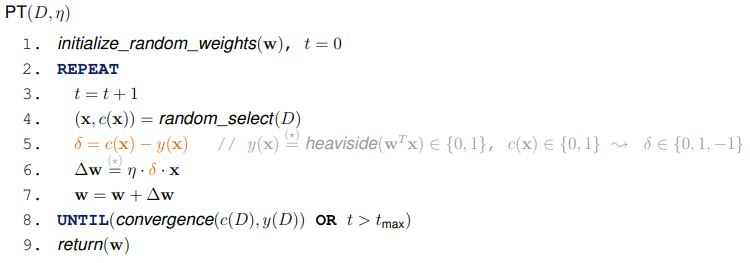
\includegraphics[width=\textwidth]{PT}
\begin{itemize}
\item If a separating hyperplane between $X_0$ and $X_1$ exists, the PT algorithm will
converge. If no such hyperplane exists, convergence cannot be guaranteed.
\item A separating hyperplane can be found in polynomial time with linear
programming. The PT Algorithm, however, may require an exponential
number of iterations.
\item Classification problems with noise are problematic
\end{itemize}
\subsection{Gradient Descent}
\begin{itemize}
\item Finde den kürzesten Weg in ein Min/Max über partielle Ableitungen
\item The gradient of a function is the direction of steepest ascent or descent.
\item in der VL ist ein Beweis den ich nicht abtippe weil irrelevant 
\end{itemize}
\subsubsection{Linear Regression + Squared Loss}

$$ L_2(\textbf{w}) = \dfrac{1}{2} \cdot \displaystyle\sum_{(\textbf{x}, c(\textbf{x})) \in D} (c(\textbf{x}) - y(\textbf{x}))^2$$

Jetzt müssen wir für jedes $w_i$ aus \textbf{w} eine partielle Ableitung machen um den weight vector zu updaten ($ \textbf{w} = \textbf{w} + \Delta \textbf{w}$)

$$ \Delta\textbf{w} =  \dfrac{ \delta }{\delta w_i} L_2 (\textbf{w}) = \eta \cdot \displaystyle\sum_D (c(\textbf{x}) - \textbf{w}^T\textbf{x}) \cdot \textbf{x}$$

$\eta$ = learning rate - a small positiv constant - legen wir selbst fest

\subsubsection{The Batch Gradient Descent (BGD) Algorithm}
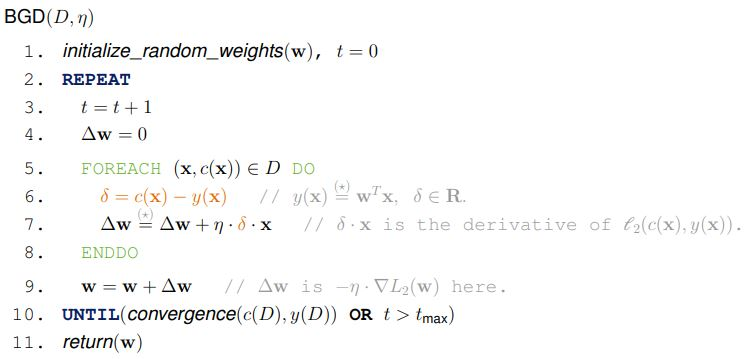
\includegraphics[width=\textwidth]{BGD}
\begin{itemize}
\item wichtig: immer wenn irgendwo $\textbf{w}^T\textbf{x}$ steht haben wir $x_0 = 1$ zu \textbf{x} hinzugefügt
\item funktionsweise BGD. wir berechnen über die Ableitung in welche Richtung wir müssen und gehen dann einen Schritt der große $\eta$
\item die "convergence" schaut ob der Squared Loss noch größer als ein $\varepsilon$ ist (das wir auch festlegen)
\item BGD ist nicht der schnellste (bestenfalls linear) aber sehr einfach (Newton-Raphson algorithm, BFGS algorithm sind z.B. schneller)
\item BGD nimmt den global loss: loss of all examples in D (“batch gradient descent”)(Schritt in Richtung die für alle Punkte am besten ist)
\item man kann auch den (squared) loss in Bezug auf einzelne Beispiele nehmen (pointwise loss) (dann gehts halt im Zickzack runter)
\ berechnet sich dann $\ell_2(c(\textbf{x}), y(\textbf{x})) = \dfrac{1}{2} (c(\textbf{x})- \textbf{w}^T\textbf{x})^2$
\item bzw. die weight adaptation: $ \Delta\textbf{w} = \eta \cdot (c(\textbf{x}) - \textbf{w}^T \textbf{x}) \cdot \textbf{x} $
\item für $BGD_\sigma$ wird Zeile 9 zu  \\ $\textbf{w} = \textbf{w} + \Delta \textbf{w} + \eta \cdot 2 \lambda \cdot \binom{0}{\overrightarrow{\textbf{w}}}$
\end{itemize}
\subsubsection{The Incremental Gradient Descent IGD Algorithm}
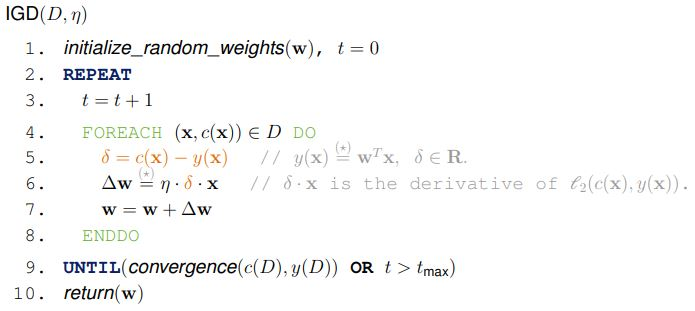
\includegraphics[width=\textwidth]{IGD}
\begin{itemize}
\item kleinere Schritte als BGD
\item  can better avoid getting stuck in a local minimum of the loss function then BGD
\end{itemize}
\subsubsection{Linear Regression + Squared Loss}
$$ L_{0/1}(\textbf{w}) = \displaystyle\sum_D \dfrac{1}{2} \cdot (c(\textbf{x})  - \sign (\textbf{w}^T \textbf{x} )) $$

$L_{0/1}8\textbf{w})$ cannot be expressed as a diffrentiable function alias es kann nicht abgeleitet werden damit ist gradient descent nicht möglich

\subsubsection{Logistic Regression + Logistic Loss + Regularization}
Wie oben nur mit neuer Formel für $\Delta \textbf{w}$:
$$ \Delta\textbf{w} = - \eta \cdot \nabla \mathcal{L}_\sigma (\textbf{w}) = 
\eta \cdot \displaystyle\sum_D (c(\textbf{x}) - \sigma (\textbf{w}^T\textbf{x}))\cdot \textbf{x} - \eta \cdot 2 \lambda \cdot \binom{0}{\overrightarrow{\textbf{w}}} $$

logistic loss Formel:

$$ \mathcal{L}_\sigma (\textbf{w} ) = \displaystyle\sum_D -c(\textbf{x}) \cdot \log(y(\textbf{x}))- (1 - c(\textbf{x}) ) \cdot \log (1 - y (\textbf{x} )) + \lambda \cdot \overrightarrow{\textbf{w}}^T \overrightarrow{\textbf{w}}  $$

\subsection{Multilayer Perceptron}
\subsubsection{Linear Separability}
2 Klassen sind teilbar wenn ich da eine gerade Linie / Ebene / Hyperplane dazwischen packen kann.... oder: \\
Two sets of feature vectors, $X_0$, $X_1$, sampled from a $p$-dimensional feature space \textbf{X},
are called linearly separable if p+1 real numbers, $w_0, w_1, . . . , w_p$, exist such that the
following conditions holds:
\begin{itemize}
\item[1.] $ \forall \textbf{x} \in X_0: \sum_{j=0}^p w_jx_j < 0 $
\item[2.]  $ \forall \textbf{x} \in X_1: \sum_{j=0}^p w_jx_j \geq 0 $
\end{itemize}

Problem: viele Probleme sind nicht linear separierbar
Lösung: wir zeichnen mehrere Linien! (nehmen multilayer perceptron)
\begin{itemize}
\item The first, second, and third layer of the shown multilayer perceptron are called input, hidden,and output layer respectively
\item  input units perform no computation but only distribute the values to the next
layer
\item Compared to a single perceptron, the multilayer perceptron poses a significantly more
challenging training (= learning) problem, which requires continuous (and non-linear)
threshold functions along with sophisticated learning strategies.
\item a continuous and non-linear threshold function: 
$$ \sigma(z) = \frac{1}{1+ e^{-z}} \Rightarrow \frac{\delta \sigma (z)}{\delta z} = \sigma(z) \cdot (1- \sigma(z)) $$
\item und damit: $ y(\textbf{x}) = \sigma (\textbf{w}^T\textbf{x}) = \dfrac{1}{1+e^{-\textbf{w}^T\textbf{x}}} $
\item eine Alternative zu $\sigma$ ist: \\
$$ \tanh (z) = \frac{e^z - e^{-z}}{e^z + e^{-z}} = \frac{e^{2z}-1}{e^{2z}+1}$$ 
\item A “multilayer” perceptron with linear threshold functions can be expressed as a single linear
function and hence is equivalent to the power of a single perceptron only $\Rightarrow$ Employing a nonlinear is necessary
\item  Multilayer perceptrons are also called multilayer networks or (artificial) neural network
\item 
\end{itemize}
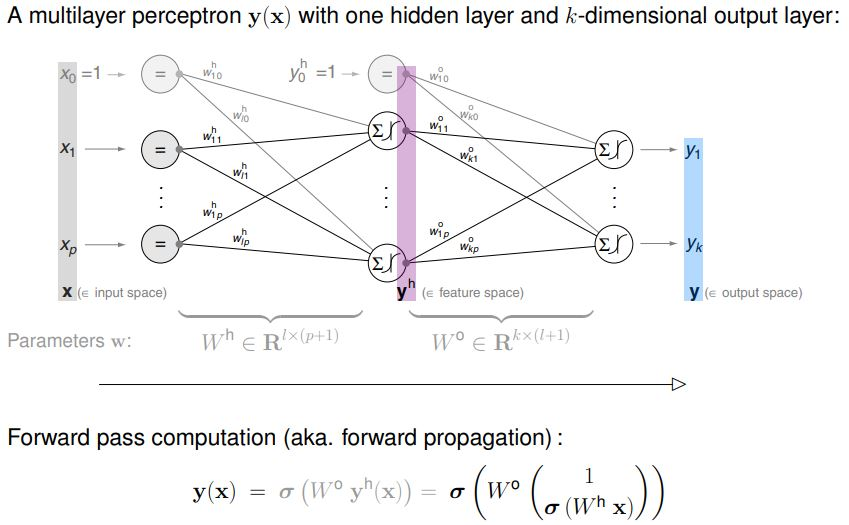
\includegraphics[width=\textwidth]{MP}
\subsubsection{Forward propagation}
The input data is fed in the forward direction through the network. Each hidden layer accepts the input data, processes it as per the activation function and passes to the successive layer
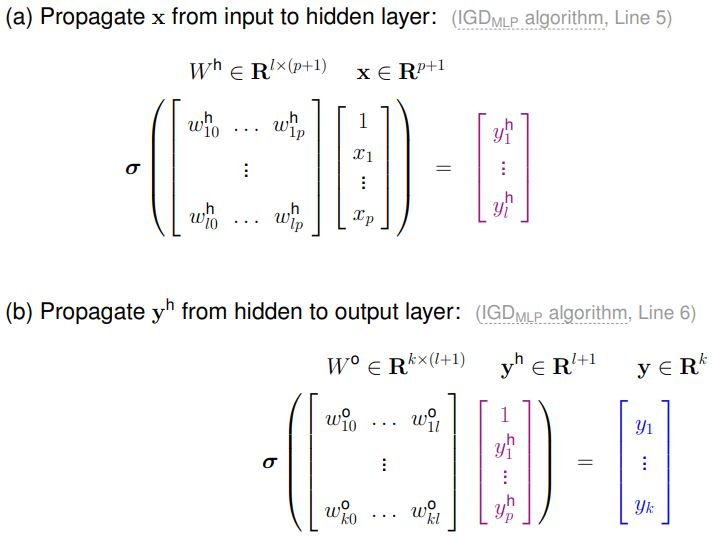
\includegraphics[width=\textwidth]{forwardProp}
\textbf{Forward propagation: Batch Mode}
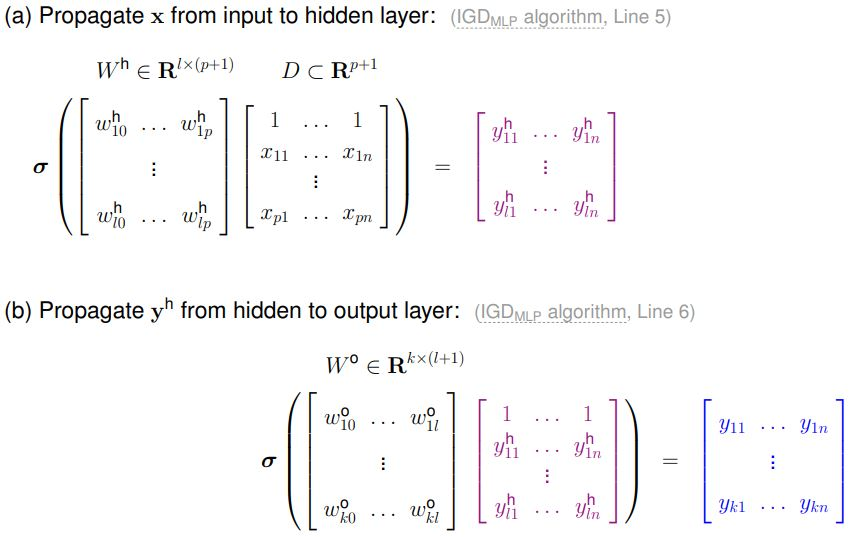
\includegraphics[width=\textwidth]{forwardPropBatch}
\subsubsection{Backwards Propagation}
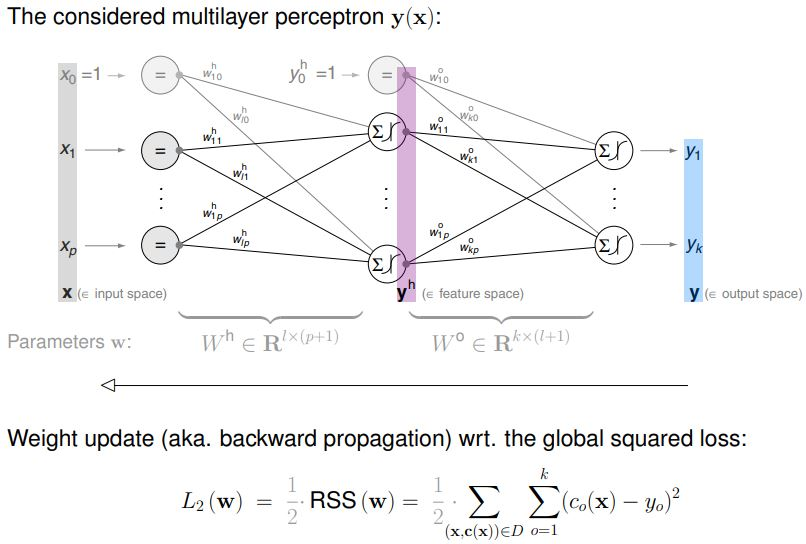
\includegraphics[width=\textwidth]{BackwardProp}
\begin{itemize}
\item $L_2 (\textbf{w})$ usually contains various local minima

\end{itemize}
\end{flushleft}
\end{document}
